%************************************************
\chapter[Persistence and biotic interactions]{The effect of multiple biotic interaction types on species persistence}\label{ch:model}
%************************************************

%\tikz[remember picture,overlay] \node[opacity=0.3,inner sep=0pt] at (current page.center){\includegraphics[width=\paperwidth,height=\paperheight]{./Figures/cover/n_pared_2.jpg}};
\tikz[remember picture,overlay] \node[opacity=0.3,inner sep=0pt] at ([yshift=3cm,xshift=2cm]current page.center){\includegraphics[width=\paperwidth,height=\paperheight]{./Figures/cover/n_pared_2.jpg}};
\clearpage

\section*{Abstract}
No species can persist in isolation from other species, but how biotic interactions affect species persistence is still a matter of inquiry. Is persistence more likely in communities with higher proportion of competing species, or in communities with more positive interactions? How do different components of community structure mediate this relationship? We address these questions using a novel simulation framework that generates realistic communities with varying numbers of species and different proportions of biotic interaction types within and across trophic levels. We show that when communities have fewer species, persistence is more likely if positive interactions—such as mutualism and commensalism—are prevalent. In species-rich communities, the disproportionate effect of positive interactions on persistence is diluted and different combinations of biotic interaction types can coexist without affecting persistence significantly. We present the first theoretical examination of how multiple-interaction networks with varying architectures relate to local species persistence, and provide insight about the underlying causes of stability in communities.

\section{Introduction}

Persistence of multicellular organisms depends on interactions with other organisms, whether they be in the form of energy intake, use of habitats created by other species, assistance in reproduction by directed dispersal of genetic material, or countless other examples \citep{Bascompte2007}. Ecological communities can be represented as networks, whereby species or guilds are nodes connected by links representing interactions \citep{Proulx2005}. Pairwise direct interactions can have positive, negative or neutral effects on the species involved, and this classification gives rise to five general types of interactions: amensalism (-,0), antagonism (+,-), commensalism (+,0), competition (-,-) and mutualism (+,+). Despite the wealth of empirical observations of biological interactions in nature, there still exists limited understanding of the frequency with which different types of biotic interactions occur in communities, and the consequences for community structure and functioning. For example, is the frequency of interaction types in communities related to overall persistence of species locally? Does the structure of the different interaction types play a role in increasing the odds of species persistence? Answering these and other questions has been hampered by difficulties in simultaneously sampling different interaction types in natural systems. Consequently, most studies have been based on observations of single interaction types within networks, which obviously has limited the ability to generalize beyond particular cases.

This fundamental gap in the understanding of ecological networks has been largely acknowledged \citep{Strauss2004, Agrawal2007, Ings2009, Fontaine2011}, and there is increasing evidence that accounting for different interaction types generates novel insights on the structure and dynamics of ecological communities \citep{Pilosof2017, Garcia-Callejas2018}.  Analyses of networks with multiple interaction types have already been applied, for example, to investigate the distribution of the different interaction types and its relationship with species traits \citep{Kefi2015,Kefi2016a} or the robustness of communities to local extinctions and habitat loss \citep{Pocock2012,Evans2013a}. Recent studies have also focused on investigating the relationship between the diversity of interaction types and several facets of community stability, often reaching different conclusions over this relationship. For example, it has been proposed that 1) mixing of interaction types generally increases local stability of model communities \citep{Mougi2012,Mougi2014,Kondoh2015}, 2) mixing of interaction types generally decreases local stability of model communities or increases the number of functional extinctions \citep{Suweis2014,Sellman2016}, or 3) structural factors of the different sub-networks enhance or decrease their stability \citep{Melian2009,Sauve2014,Sauve2016}. The conflicting results over this fundamental question can be explained by the sheer diversity of modeling assumptions, structural constraints, and varying sets of interaction types included in the studies. For example, several studies \citep{Melian2009,Sauve2014,Sauve2016} analyzed communities consisting of only antagonistic and mutualistic interactions in which a central group of species (usually plants) is the guild connecting the mutualistic (e.g. plant-pollinator) and antagonistic (e.g. plant-herbivore) networks. Other studies considered model communities with only basic rules about food web structure \citep{Mougi2012,Suweis2014}. A common feature of most studies is that, with the exception of \cite{Mougi2016a}, their models did not consider the five general interaction types concurrently. However, \cite{Mougi2016a} only analyzed random interaction matrices in his model, making his conclusions difficult to contrast with those of other studies that assumed stronger structural constraints. The role of species richness in mediating community stability also has been extensively studied in single-interaction networks, and analytical derivations have been produced for idealized conditions in mutualism-competitition networks \citep{Allesina2012}. In most cases, theory shows that increasing richness decreases local stability of random networks, but it is unclear how species richness mediates different facets of stability in networks with more complex structures and varying proportions of interaction types.

All in all, while approaches assessing the local stability of random interaction networks have important heuristic value \citep{Allesina2012,Allesina2015}, such randomly assembled networks lack key structural patterns found in real communities \citep{Jacquet2016}. Furthermore, local stability analyses have little concordance with non-equilibrium dynamics of real systems \citep{Pimm1982,Chen2001}, which limits their predictive ability. The equilibrium assumption is further ingrained in most interaction models by assuming that interactions occur with a constant strength coefficient. This assumption is widely used for convenience despite repeated claims against its realism \citep{Abrams1980,Abrams2001,Hernandez1998,Holland2009}. Here we address all the above-mentioned shortcomings and investigate whether the frequencies of the five biotic interaction types affect persistence of species in communities with varying species richness. We generate model networks informed by empirical observations on distributions of species abundances across trophic levels, link topology, and develop a measure of the impact that a species has over another based not on static interaction coefficients, but on species abundances and their associated frequency of interaction. With this model design, and by performing a comprehensive set of simulations, we ask the following questions: 1) Is species persistence affected by the frequency of the different interaction types in model communities? If so, does community richness mediate this relationship? 2) Which types of biotic interactions are more likely to be lost, as species go locally extinct? Lastly, given the unfeasibility of validating our predictions with empirical data, we indirectly test the validity of our model by asking: 3) does our model generates community-level patterns consistent with those of empirical networks?

\section{Methods}

We designed a dynamic network model accounting for the five possible types of pairwise interactions (antagonism, amensalism, commensalism, competition, and mutualism), whereby the impact of a species over another is characterized by the abundances of the species involved. Accounting for different interaction types meant that a trophic level distribution of species had to be specified a priori, as we expected different interaction types to be distributed unevenly across trophic levels. Furthermore, the modeling of pairwise interactions in our model is closely linked to the abundances of the interacting species, so we imposed non-random initial abundance values. In particular, we assembled our model communities with three assumptions:

1) The initial Species Abundance Distribution of the overall community follows a hollow curve.


2) The initial abundances of the different trophic levels vary with a power-law scaling.


3) The distribution of interaction types within and across trophic levels is non-random.


In the following sections, we describe these assumptions and the methodology for incorporating them in the community assembly process. Then, we specify the implementation of the dynamic interactions model and the simulations performed. The main response variable obtained from our simulations is the ratio of persistent species in our model networks. Thus, in the context of the present study, we define community persistence as the ratio between initial (denominator) and final (numerator) number of species in a simulated community. Persistence values can therefore range from 0 (all initial species have died out by the end of the simulation) to 1 (all species show positive abundances at the end of the simulation).

\subsection*{1) Abundance distribution of the overall community}

Each species within a model community was assigned an initial abundance by drawing random samples from a gambin distribution. The gambin is a distribution with a single free parameter that provides a similar or better fit to empirical SADs than classic choices such as the lognormal or the logseries \citep{Matthews2014a}. A value of $\alpha = 2$ was given to generate the initial SADs.

\subsection*{2) Abundance scaling across trophic levels}

Species were distributed among four trophic levels (a basal one consisting on primary producers and three consumer levels), which is a number commonly found in empirical communities \citep{Ulanowicz2014a}. Assignment of species into each trophic level was made following the findings of \cite{Hatton2015}, who showed that for herbivore-predator trophic guilds, biomass distribution follows a power law with exponent ~ 0.75. These authors generalized the scaling rule to the abundance of species at each trophic level since, for most predator-prey couplings, weak relationships between body mass and community biomass were found. As a starting working hypothesis for the simulations, we extended Hatton’s et al (2015) scaling rule to the four trophic levels considered.

\subsection*{3) Distribution of interaction types within communities }

The different types of biotic interactions are unlikely to be uniformly distributed in nature. Yet little is known regarding the varying proportion of interaction types within communities or trophic levels \citep{Dodds1997}, let alone about changes in such proportions across communities, or the effects of varying proportions of interaction types on mechanisms of community assembly.

A first step towards examining the frequency distribution of the different interaction types in a community with several discrete trophic levels is to consider the sign matrix of the community, $S$, assuming that interaction signs are kept constant within the spatial and temporal limits of the study, and with varying abundances. We hypothesize that the relative frequency of each interaction type in S will be influenced by the number of species in the different trophic levels, as different interaction types will have different probabilities of occurring among species belonging to the same or different trophic levels. In order to check this working hypothesis, we undertook an extensive survey of literature on biotic interactions and compiled the extent to which the five general interaction types (amensalism, antagonism, commensalism, competition, mutualism) are documented to occur between species of the same, adjacent, or non-adjacent trophic levels. Specifically, we performed a search in the Web of Science for studies published from 1991 to 2015, including the terms “ecology” AND “interaction” AND “interaction type” (see also \citealt{Morales-Castilla2015}). We reviewed studies documenting direct pairwise interactions and annotated the trophic level of the species involved. For competition, antagonism (predation OR herbivory), and mutualism, we included \textit{ca}. 100 papers. For commensalism and amensalism the list of suitable studies was more reduced (67 studies on commensalism and only 12 on amensalism). We constrained the results by discarding interactions involving microorganisms, fungi, parasites or parasitoids, owing to the overall difficulty of classifying these groups into clear cut trophic levels. The list of selected studies is available as online supplementary material in the published article, see section \textit{Chapter references} for the full reference. The resulting relative frequencies (Fig. \ref{fig:fig3.1}) were incorporated as a last constraint in the model in the form of probabilities of pairwise interactions taking place within a single trophic level, adjacent, or other trophic levels.

For estimating the number of links of each species, we followed the constant connectance hypothesis \citep{Martinez1992}. Thus, we assumed no variation in connectance levels with initial community size, imposing C = 0.5 for every simulation, where connectance is defined as the ratio between realized and potential interactions in the network. This value was chosen so that specific connectances of the different interaction types (see Appendix 3.4) ranged between 0.07 and 0.2, values consistent with empirical estimates of mutualistic and antagonistic connectance \citep{Thebault2010}.

With the probabilities of interaction occurrence across trophic levels (Fig. \ref{fig:fig3.1}) and connectance values of the network, we constructed the sign matrices of our model communities stochastically: for each link, first its interaction type is selected; second, the trophic levels affected by that interaction are chosen according to the probabilities of interaction occurrence; and third, the specific species are randomly chosen. This process ensures that, on average, sign matrices will reflect the probabilities of Fig. \ref{fig:fig3.1}, while allowing for an intrinsic component of variability in each particular matrix. The full community assembly process is explained in detail in Appendix 3.1.

\begin{figure}[!ht]
\centering
\includegraphics[width=.5\textwidth]{./Figures/chapter03/Fig_1.png}
\caption[Interaction occurrences across trophic levels]{\color{Gray} relative frequency of trophic levels involved in pairwise interactions for each interaction type. When the trophic level of the interacting species was not explicitly alluded to, we assumed that 1) species of the same taxonomic group belong to the same trophic level (e.g. isopods), 2) omnivory represents feeding on both “adjacent” and “other” trophic levels, 3) pollinators and seed dispersers are “adjacent” to plants. $N_{amensalism} = 12$, $N_{antagonism} = 135$ (123 of adjacent trophic levels, 10 of other, 2 of same), $N_{commensalism} = 65$ (44 of same trophic level, 20 of adjacent, 1 of other), $N_{competition} = 97$ (95 of same trophic level, 2 of adjacent), $N_{mutualism} = 113$ (94 of adjacent trophic levels, 11 of same, 9 of other).}
\label{fig:fig3.1}
\end{figure}

\subsection*{A framework for modeling dynamic interactions}

The realization and outcome of direct pairwise interactions is dependent on three classes of mechanisms \citep{Poisot2015}: First, the frequency of stochastic encounters of individuals mediated by their relative abundances. Second, the matching of traits between individuals that establish contact. Third, other factors such as environmental constraints or the influence of higher order interactions with other species. Hence, empirical measurements of interactions show a high degree of variability explained, partly, by density-dependent mechanisms \citep{Aizen2014}, by trait matching \citep{Santamaria2007} or by environmental factors \citep{Mazia2016,Poisot2017}. This inherent variability on both the sign and the strength of interactions has hardly been explored in community dynamic models, even if the assumption of static interaction sign and strength is known to be unrealistic \citep{Abrams1980,Abrams2001,Hernandez1998,Holland2009}. The importance of each mechanism in explaining observed patterns of interaction strengths is currently under debate. In plant-pollinator networks, for example, the net impact of a species over another is significantly related to the frequency of interaction \citep{Vazquez2005,Vazquez2012}, and to the abundances of the interacting species \citep{Vazquez2007}, but not in all cases. A neutral model of interactions can also reproduce structural patterns observed in empirical food webs \citep{Canard2012}. On the other hand, trait-matching has been shown to accurately reproduce network structure in different types of networks \citep{Eklof2013}, and also outperforms neutral interaction frequency for predicting network structure in some empirical networks \citep{Vizentin-Bugoni2014,Sazatornil2016}. However, another recent study showed that while abundances and traits can predict network structural patterns, they were not generally able to predict the realization of specific interactions in a plant-pollinator network \citep{Olito2014}. Finally, higher-order influences on interaction occurrence and strength, in particular environmental forcing, are a main focus of Stress Gradient Theory \citep{Maestre2009} and Environmental Stress Models \citep{Menge1987}, but an integration of these frameworks with the recent advances on multi-trophic, multiple interactions networks is still lacking.

We modeled the impact of a species over another by considering the first of these three mechanisms, i.e. the stochastic encounters between individuals of two populations driven by their abundances. This process is the only one that can be generalized to any interaction and community type without considering further, specific assumptions about trait distributions or the role of environmental covariates. Thus, in our modeling framework, the impact of a species over another is only dependent on the frequency of interaction between the two species, which in turn depends on their net abundances. As our approach is fundamentally different to that of models with static interaction strength coefficients, we refer to the interaction strength in our model as species impact (a population-level effect, \citealt{Vazquez2012}).

In formulating species impact, we followed \cite{Poisot2015} and considered it a product of interaction frequency by an interaction strength term:

\begin{equation} \label{eq:eq3.1}
I_{i,j} = IF_{i,j} * IS_{i,j}
\end{equation}

The $IF$ function derives the net frequency of interactions between two populations in a given time interval from their local abundances. We assume that (1) the maximum potential interaction frequency will equal the population density of the least abundant species, and (2) interaction frequency saturates asymptotically, as one or both abundances increase. It takes the form:

\begin{equation} \label{eq:eq3.2}
IF_{i,j} = min(N_i,N_j) \frac{1}{1 + e^{-a(max(N_{i},N_{j}) - x_0)}}
\end{equation}

The $a$ parameter adjusts the saturating behavior of the function (i.e. its steepness), so that a higher value of a implies that the $IF$ function saturates at lower abundances of both populations, i.e. interactions are comparatively more common. Parameter $x0$ indicates the abscissa of the midpoint for the logistic part of the function, and was kept for reference.

The $IS$ function (for interaction strength) models the sign and strength of per capita interactions of species $j$ over species $i$. This function was defined just as the sign of the pairwise interaction times a scaling factor for differentiating interaction types. For example, a scaling of 1 indicates that the maximum effect of species $j$ over species $i$ is of the same order of magnitude as the population growth rate. Therefore, we defined the $IS$ function simply as:

\begin{equation} \label{eq:eq3.3}
IS_{i,j} = s_{i,j} * k_t
\end{equation}

where $s_{i,j}$ is the sign of the effect of species $j$ over species $i$, and $k_t$ is the scaling factor for an interaction of type $t$.

We incorporated Eq. \ref{eq:eq3.1} to a population dynamics model based on the recent extensions to the logistic growth equation by \cite{Garcia-Algarra2014}. Their formulation averts a known divergent behavior of the r-k classic form of the logistic equation and is sufficiently simple while being able to reproduce the complexity of more elaborate models in terms of fixed points and stabillity of the dynamics. Consider a community of $n$ species. The model has the form:

\begin{equation} \label{eq:eq3.4}
\frac{dN_i}{dt} = r_i N_i
\end{equation}

whereby all extrinsic effects – environmental, biotic interactions – fall on the intrinsic growth rate $r_i$. This allows the comparison between the strength of different interactions, i.e. it is an example of an equal footing network \citep{Garcia-Callejas2018}. The effective growth rate is modeled as:

\begin{equation} \label{eq:eq3.5}
r_i=r_i^0+\sum_{j=1,j{\neq}i}^n I_{i,j} - (\alpha_i + c_i \sum_{j=1,j{\neq}i}^{n} I_{i,j})N_i
\end{equation}

where $r_{i}^{0}$ is the intrinsic growth rate, $\alpha_i$ is the friction term that regulates the asymptotic behavior of the function, $c_i$ is a proportionality constant, and $I_{i,j}$ is the impact function from Eq. \ref{eq:eq3.1}.

\subsection*{Simulations}

We generated theoretical communities with 20,40, and 60 initial numbers of species that corresponded to overall abundances of around 2395, 4640 and 6850 individuals, respectively. For each richness level, we defined six types of communities according to the frequency with which the different interaction types occurred: equal ratio type with relative frequency of 0.2 for every interaction type; and five types in which each of the interaction types was the most prevalent (with frequencies of 0.4 for the prevalent type and 0.15 for the others). We projected the dynamics of 1000 replicates for each of these combination of factors, ending up with $3*6*1000 = 18000$ simulated communities. For each replicate, aside from the inherent stochasticity of the assembly process, we drew the intrinsic growth rates and saturation terms of each species ($r_{i}^{0}$ and $\alpha_i$ from eq. \ref{eq:eq3.5}) randomly from an interval of potential values (Appendix A.3.1: Table A.3.1.4), ensuring that primary producers have intrinsic growth rates $r_{i}^{0} > 0$ and consumers $r_{i}^{0} < 0$. Introducing these stochastic components on the assembly process and parameterization enabled us to test the robustness of the model to small variations in its initial conditions. The full parameterization of the model, alongside with further details about its implementation and numerical solving, is given in Appendix 3.1. Preliminary tests showed that most simulated communities reached a stable abundance distribution after 2500 or less time steps but, conservatively, we ran our dynamic model for 5000 time steps. In order to be more confident on the time steps chosen, we also tested whether there were significant differences between the resulting persistence patterns after 5000 and 10000 time steps. As no significant differences were found, we considered 5000 time steps to be an appropriate time frame for our simulations.

We also performed additional simulations in order to test the influence of the imposed structural constraints in our results. In these simulations we relaxed, one by one, the three constraints of the community assembly process (see Appendix 3.3 for more details).

\section{Results}

\subsection*{Is species persistence influenced by the frequency of the different interaction types? If so, does community richness mediate this relationship? }

Model communities with a higher proportion of positive interactions (mutualism and, to a lesser extent, commensalism) tended to have higher species persistence than any other community type (Fig. \ref{fig:fig3.2}, results of statistical tests in Appendix A.3.2: Table A.3.2.1 and Table A.3.2.2). The effect of positive interactions on persistence was strongest for species-poor communities, and decreased consistently as the numbers of species in the communities increased. Although average species persistence converged to around 88\% as richness increased, there was significant variation between the persistence of species belonging to the different trophic levels (Appendix A.3.2: Figure A.3.2.1): in communities with low initial richness, the second and third trophic levels saw more extinctions than the first, while species on the fourth trophic level did not show a uniform behavior, and were more dependent on variations in the relative frequency of interaction types. This general pattern was reversed in more speciose communities, in which species of all higher trophic levels showed more persistence than the basal ones, for all community types.

Supplementary simulations (Appendix A.3.3) showed that persistence values are further influenced by the community structural patterns imposed. The removal of both the abundance scaling across trophic levels and the distribution of interaction types across trophic levels had a significant negative effect on persistence. Sampling species abundances from a uniform SAD instead of a skewed one, on the other hand, increased overall persistence.

\begin{figure}[!ht]
\centering
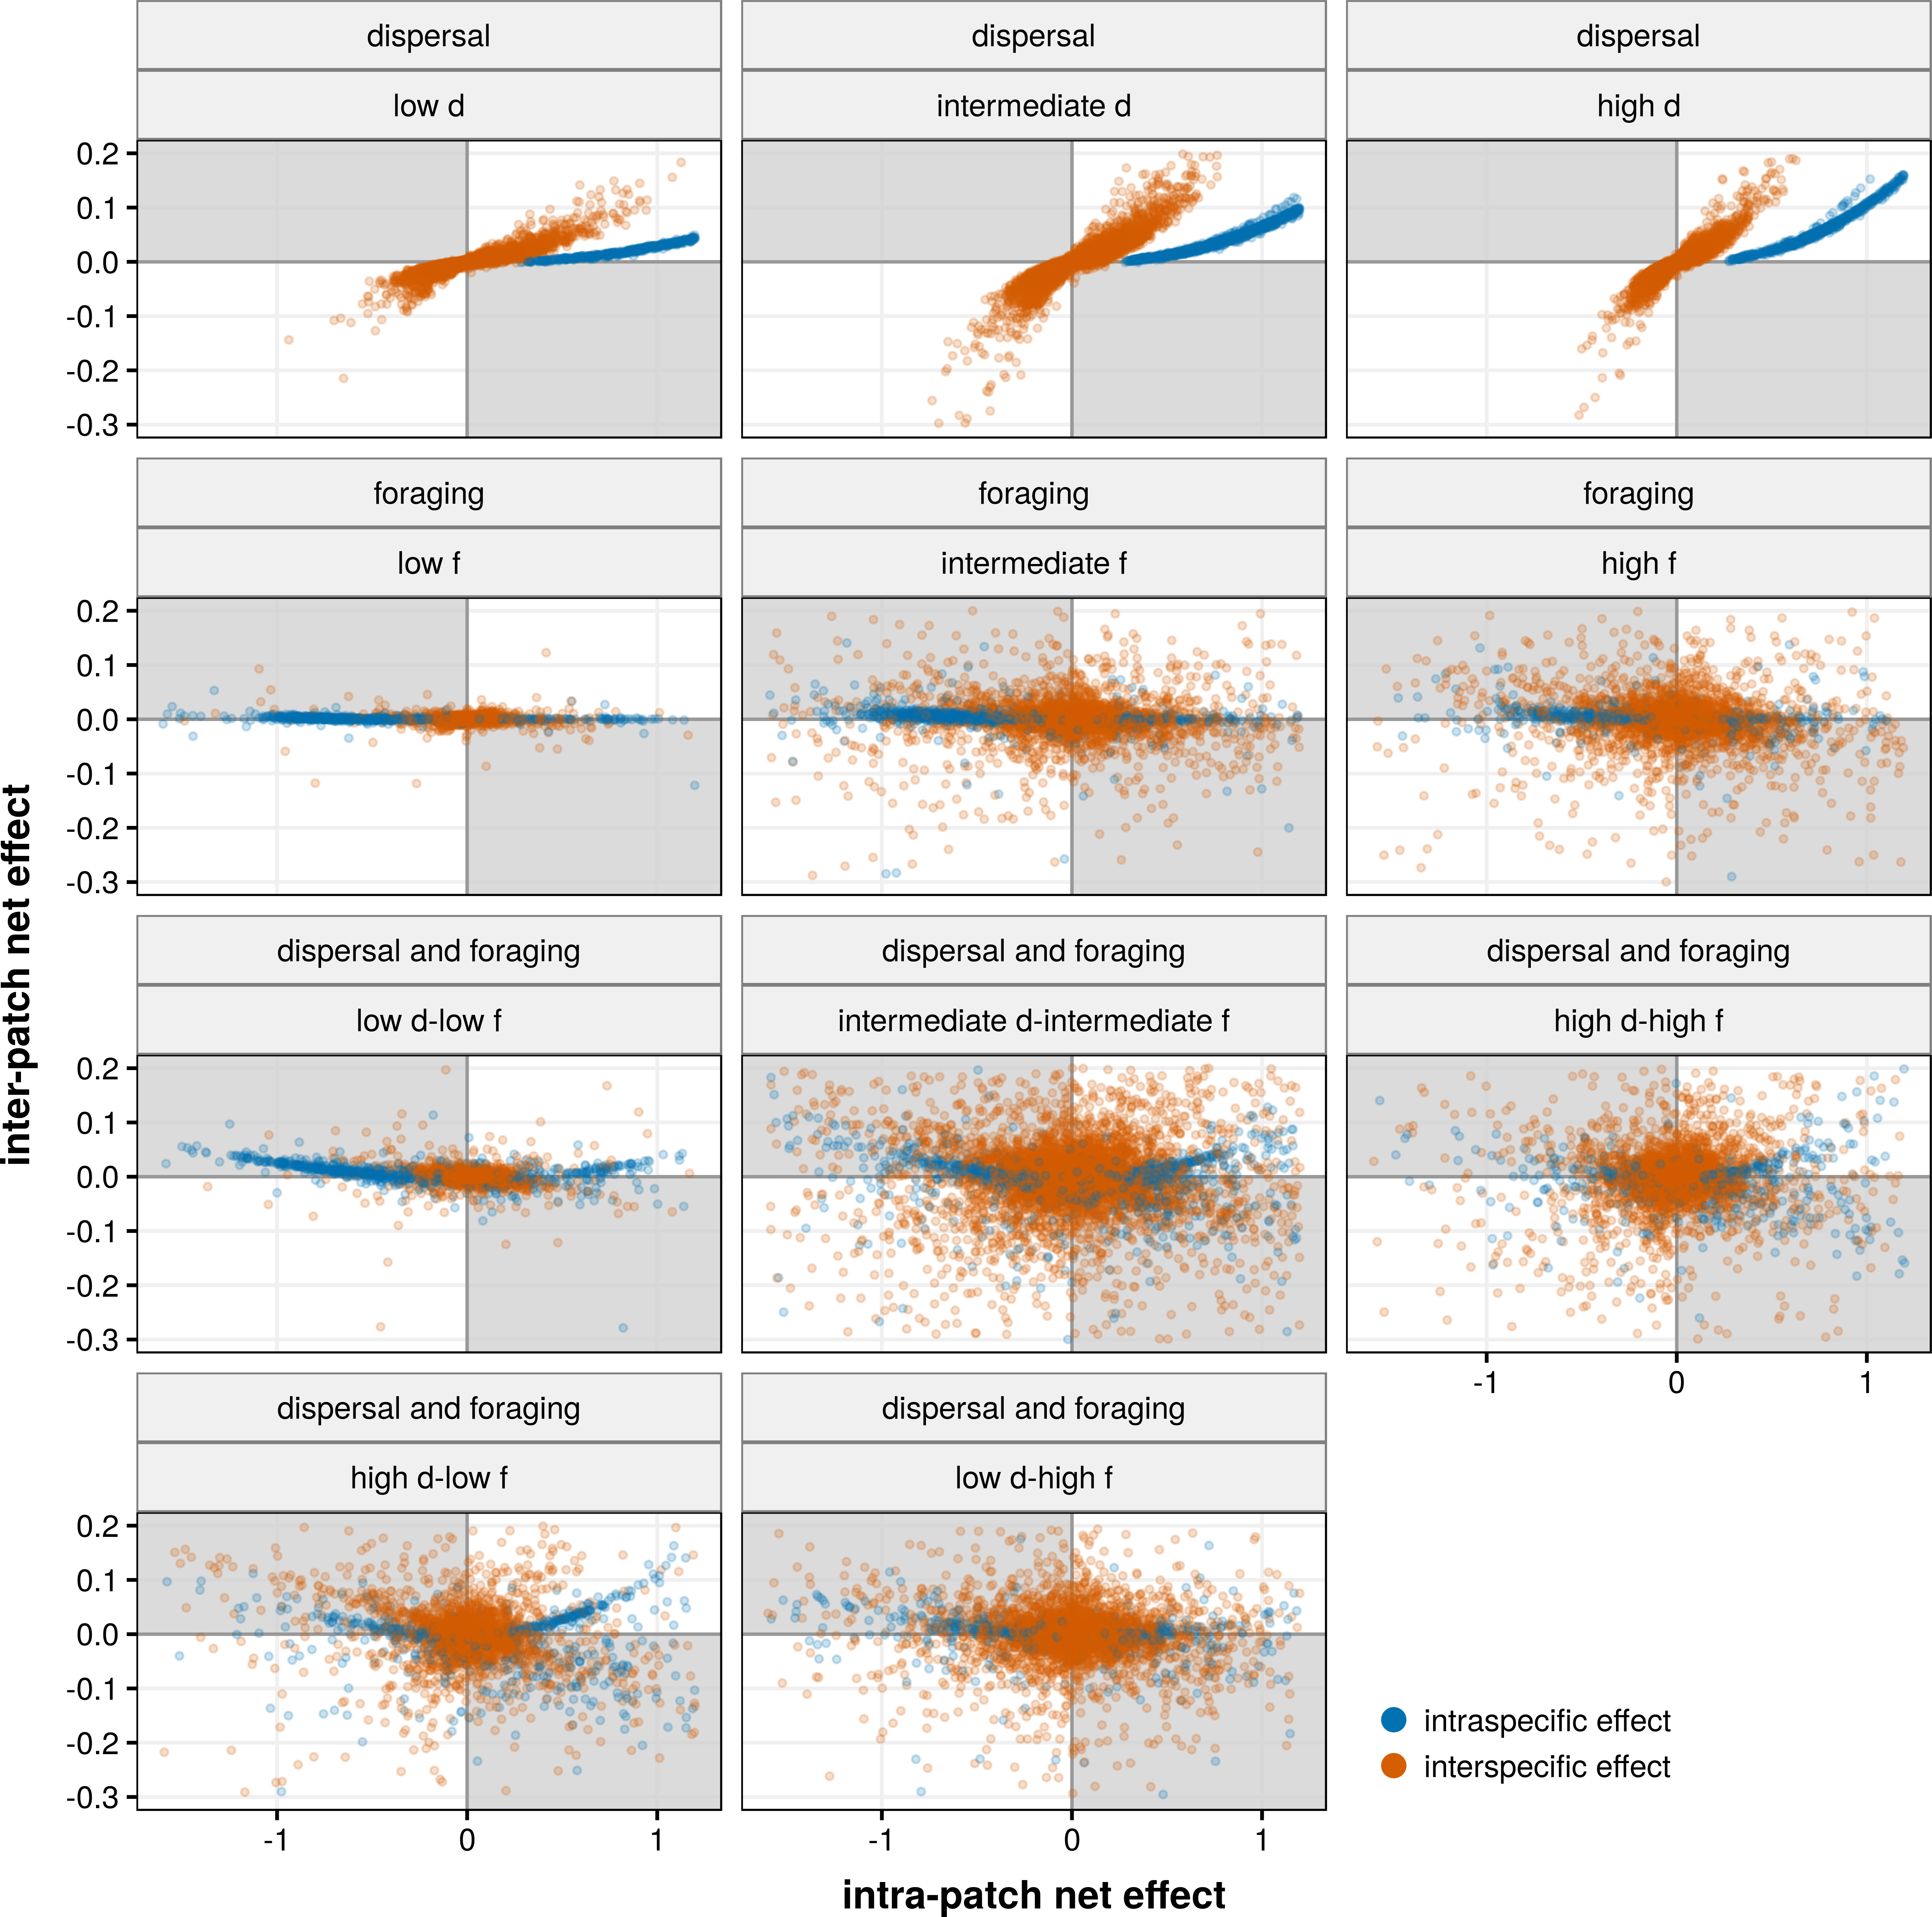
\includegraphics[width=\textwidth]{./Figures/chapter03/Fig_2.png}
\caption[Persistence of model communities]{\color{Gray} Persistence values of the simulated communities at the end of the simulations. Vertical axis represents the relative frequency of a given persistence value in the pool of replicates (1000 replicates for every combination of initial richness and initial frequency of interaction types). All resulting pairs of persistence distributions but one are significantly different according to Kruskal-Wallis rank tests (Appendix A.3.2: Table A.3.2.1) and post-hoc Dunn’s tests (Appendix A.3.2: Table A.3.2.2).}
\label{fig:fig3.2}
\end{figure}

\FloatBarrier

\subsection*{Which types of biotic interactions are more likely to be lost, as species go extinct?}

In our model, local extinctions have structural consequences for the remaining network: when a species goes extinct, its interactions disappear as well and are not replaced. The initial and final frequencies of the different interaction types were significantly different in most cases (Fig. \ref{fig:fig3.3}, results of statistical tests in Appendix A.3.2: Table A.3.2.3). Amensalism and competition tended to decrease in relative frequency with respect to initial levels, while mutualism tended to increase. Antagonism and commensalism responded differently for varying levels of community richness. Antagonistic interactions decreased in frequency only in communities with 20 initial species, while in communities with 60 species, they increased; the opposite was observed for commensalism, which increased in species-poor communities but decreased with high species richness.

\begin{figure}[!ht]
\centering
\includegraphics[width=\textwidth]{./Figures/chapter03/Fig_3.png}
\caption[Initial and final interaction ratios]{\color{Gray} Initial and final frequency of each interaction type in each community parameterization (rows: richness levels, columns: interaction frequencies levels). Each dot represents a single simulation, color code is the same as Fig. \ref{fig:fig3.2}. Upper left symbols in each panel represent the significance of the difference in initial and final ratios according to Wilcoxon signed rank paired tests, in black for the whole set of simulations, and colored for the simulations with high ratio of the respective type (n.s.: p-value > 0.05, *: p-value $<$ 0.05, **: p-value $<$ 0.01, ***: p-value $<$ 0.001. See Appendix A.3.2: Table A.3.2.3 for details.}
\label{fig:fig3.3}
\end{figure}

\FloatBarrier

\subsection*{Does our model reflect structural patterns observed in empirical networks?}

Focusing on the structural features listed by Jacquet et al. (2016), we checked three features observed in empirical networks: the distribution of interaction strengths (species impacts in our scheme), their variation in magnitude with trophic level, and the correlation of antagonistic pairwise interaction impacts. The distribution of species impacts in our model communities ($I_{i,j}$ in Eq. \ref{eq:eq3.1}) was positively skewed in all cases, with communities with high proportion of negative interactions being the most skewed (Fig. \ref{fig:fig3.4}, Appendix A.3.2: Table A.3.2.4). The magnitude of species impact decreased consistently with increasing trophic level (Fig. \ref{fig:fig3.4}, Appendix A.3.2: Table A.3.2.5 and Table A.3.2.6). Lastly, there was a significant negative correlation in the values of pairwise species impact for antagonistic interactions (Fig. \ref{fig:fig3.4}, Wilcoxon signed-rank tests, $V = 0$, $p < 0.001$ in all cases).

\begin{figure}[!ht]
\centering
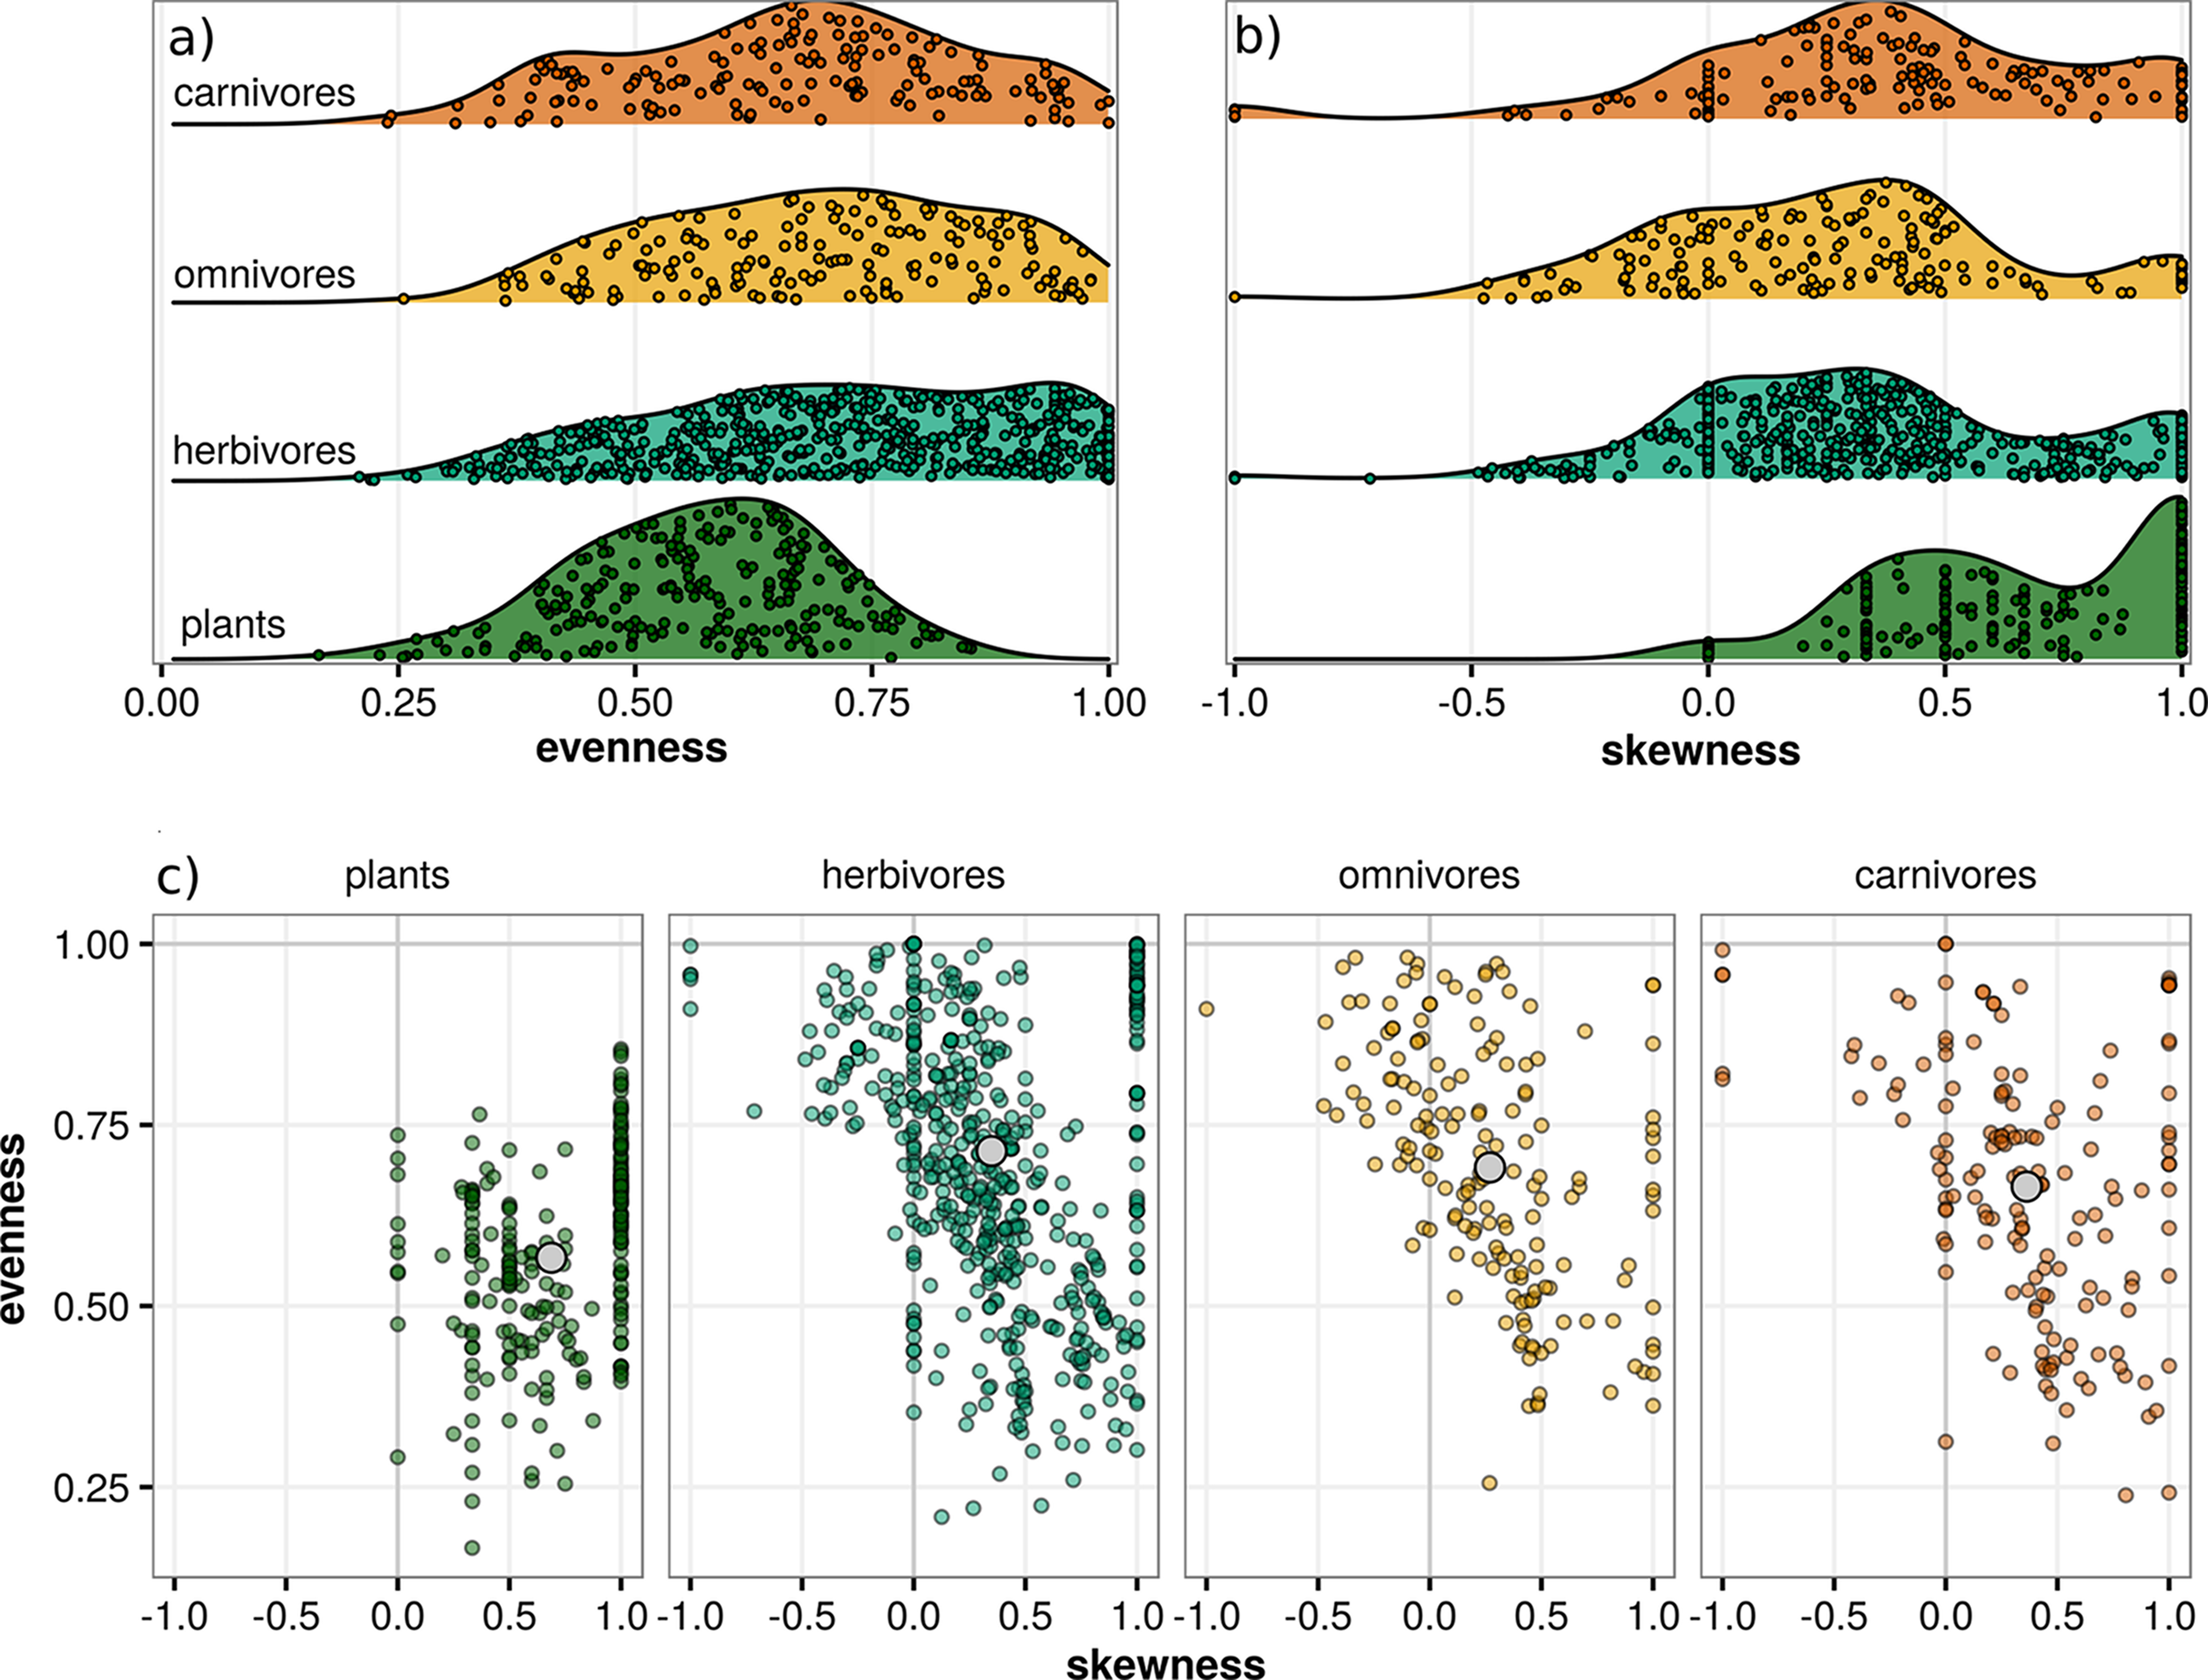
\includegraphics[width=\textwidth]{./Figures/chapter03/Fig_4.png}
\caption[Community structural patterns]{\color{Gray} Structural patterns observed in our model, at the initial and final steps of the simulations. Data shown corresponds to simulations with an initial richness of 60 species and equal probability of occurrence for every interaction type. a) Skewed distribution of species impacts. b) Decrease in average impact per trophic level (error bars represent an interval of one standard deviation centered in the mean). c) Correlation of species impact among pairs of species. In this panel, the only interactions accounted for are antagonistic ones.}
\label{fig:fig3.4}
\end{figure}

\section{Discussion}

Our simulations indicate, primarily, that positive interactions are key for maintaining species persistence, particularly in species-poor communities. For understanding the outcomes of our model and in order to place them in a general context, we first evaluate the role and implications of modeling interaction impacts based on species abundances and interaction frequencies. Secondly we analyze the combined influence of other community-level factors.

\subsection*{Species persistence and pairwise direct interactions}

All other things being equal, the number of interactions every species has with other species (i.e., their degree) is expected to increase with increasing number of species in the community. This is exactly what we recorded in our model communities: by keeping network connectance constant, we obtained average degrees of 9.5 for communities of 20 species, and degrees of 19.5 and 29.5 for communities of 40 and 60 species, respectively (values not far from the empirical estimates obtained by \cite{Kefi2015}, who reported an overall connectance of 0.47 for a community of 104 species, and thus a mean overall degree of 24.2). Given such a scenario, in species-poor communities the dynamics of a species will directly depend on only a handful of pairwise interactions. In such cases, a single interaction with high impact will have a disproportionate direct effect on species dynamics and, by extension, the prevalence of negative or positive interaction types will be an important driver of persistence at the community level.

The direct impact of interactions in communities is not only dependent on their numbers, but also on the abundances of the interacting species. Considering a skewed SAD (Species Abundance Distribution) of the overall community, as in our main simulations, the percentage of rare species (e.g. these with $<$ 10 individuals) increases and then stabilizes with increasing richness, while the percentage of very abundant species (e.g. with > 100 individuals) decreases (Appendix A.3.2: Table A.3.2.7). In species-poor communities, thus, a higher proportion of interactions will involve very abundant species, increasing the probability of comparatively strong direct impacts on species dynamics. As richness increases, more interactions will take place between comparatively rare species. The average impact per interaction will decrease accordingly (Appendix A.3.2: Figure A.3.2.2), with the effect that average persistence will increase regardless of the distribution of interaction types.

An important consequence of the differential effect of interaction types on species persistence is that species engaging in a high number of direct positive interactions will tend to persist and maintain their interactions, whereas species with a high number of direct negative interactions will tend to go extinct more frequently and, thus, their associated interactions will be lost, increasing the overall ratio of positive interactions (Fig. \ref{fig:fig3.3}). This reasoning is, however, contingent on the modeling assumption that there is no interaction rewiring. Keeping in mind this strong assumption, if these results hold, natural assemblages should be filtered to maintain a relatively high ratio of direct positive interactions, in particular in species-poor communities, and species with a high degree of negative interactions will be rare and, in any case, have otherwise strong life-history traits that allow them to persist. Note that, throughout the study, we limit our discussion to the role of direct interactions. The importance of indirect or net effects for understanding community patterns is well established (e.g. \citealt{Montoya2009a}), and the mechanisms proposed here for linking species interactions, abundance and persistence, would be improved by accounting for the role of these higher-order effects. However, in model networks, net effects are commonly analyzed by calculating the negative of the inverse Jacobian matrix \citep{Novak2016}. The formulation of our model, without static interaction coefficients and, potentially without attaining static equilibria, limits the applicability of analyses based on Jacobian matrices. Therefore, we opted not for calculating net effects and leave their analyses in our framework for future studies.

By explicitly modeling species impacts based on species abundances and interaction frequencies, our interpretation of species persistence and community dynamics differs fundamentally from that of other theoretical models of multiple interactions (e.g. \citealt{Mougi2012}). Furthermore, our response factor, species persistence, also differs from the common local stability analyses performed in the majority of theoretical network studies. Despite these fundamental differences, some common trends seem to surface. Much like our finding that the frequency of interaction types is less important in speciose communities, in the study by \cite{Mougi2012} increasing richness allowed for high local stability regardless of the proportion of positive to negative interactions (but see \citealt{Suweis2014}). With a completely different methodology, built on individual-based models, \cite{Lurgi2016} further found that increasing the proportion of mutualistic links increased overall stability in their model. Yet another, more general interaction model showed that positive interactions tend to become dominant in interaction networks as a consequence of spontaneous self-organization \citep{Jain2001}. Overall, these independent lines of evidence point to the combined importance of positive interactions and community size on stability patterns in a broad sense.

The relationship between species richness, abundances and interaction types may shed light on other general questions in community ecology, aside from the comparison with previous theoretical models.

First, in line with empirical findings from plant communities in stressful environments \citep{Soliveres2014, Cavieres2009}, we have shown that a high ratio of positive to negative interactions significantly increases species persistence, particularly in communities with low initial richness. By the explicit consideration of four discrete trophic levels, we show that a preponderance of positive interactions is particularly important for the persistence of intermediate consumers (Appendix A.3.2: Figure A.3.2.1), upper panels). These species are preyed upon by top predators and also subject to competition (both direct as modeled and indirect as a result of resource consumption) and amensalism. Hence, they are potentially the most benefited from engaging in mutualisms with species from adjacent trophic levels. As mutualistic interactions are most prevalent across adjacent trophic levels (Fig. \ref{fig:fig3.1}), intermediate species will be the ones showing a highest degree of these positive interactions. Note that we did not model competition for resources at the basal trophic level, and all our communities included a fourth trophic level of top predators. Thus, these latter species, not subject to predation (aside from a very small probability of intraguild predation, Fig. \ref{fig:fig3.1}), are likely to have a strong top-down influence on the persistence of intermediate species.

Second, our findings contribute to reframing the debate on whether pairwise interactions are stronger in richer communities. On the one hand, the hypothesis of a gradient on pairwise interaction strength with latitude has been generally supported on empirical grounds (\citealt{Schemske2009}, but see \citealt{Moles2016}), but it is unclear whether or how this pattern is affected by the richness of the analyzed communities. On the other hand, we have shown that if interaction impacts are neutral (i.e. driven solely by species abundances), then species impact will generally decrease with increasing richness. This theoretical result has been partially supported in a recent study that found that, on islands whose size granted a certain environmental stability, the strength of competitive and antagonistic interactions decreased with island size and richness \citep{Schoener2016}. Clearly, an array of factors can cause deviations from neutrality in interaction strengths (IS function in eq. \ref{eq:eq3.1}), and hence the neutral interactions hypothesis should be viewed as a baseline for estimating species impacts when no other information is available. Such neutral estimations have already been applied for plant-pollinator networks \citep{Vazquez2012} or in sampling campaigns of multiple interactions networks \citep{Pocock2012}.

\subsection*{Emerging community structure further enhances persistence}

Components of community structure, such as species diversity or different network-level metrics, have been regarded as key factors in previous modeling studies \citep{Sauve2014,Sauve2016}, where accounting for empirically informed values generally enhances stability metrics. Such theoretical results are, however, difficult to validate, since empirical data on communities with varying structural patterns is extremely scarce. As an alternative for testing the adequacy of our model, we analyzed whether our model communities displayed properties comparable to those found in empirical networks. Recently, \cite{Jacquet2016} showed that empirical food webs possess three structural characteristics that clearly differentiate them from random counterparts: first, they display the classic skewed distribution of interaction strengths, whereby there are very few strong interactions and a majority of weak ones \citep{McCann1998}. Secondly, empirical food webs show strong pairwise correlations in interaction strengths, in line with theoretical findings \citep{Tang2014}. Thirdly, interaction strengths are not evenly distributed across trophic levels; rather, average interaction strength tends to decrease with trophic level. In our model, the skewed distribution of species impacts and their “pyramidal” arrangement are observed and maintained throughout the community dynamics (Fig. \ref{fig:fig3.4}, panels A and B). On the other hand, the pairwise correlations generated in our model communities (Fig. \ref{fig:fig3.4}, panel C) are significantly different from zero but smaller than those reported by \cite{Tang2014}. Such disparity may be due to the lack of trait-matching mechanisms in our model, as trait-matching may give rise to increasingly specialized and correlated pairwise interactions \citep{Santamaria2007}.

The three patterns outlined by \cite{Jacquet2016}, i.e. skewed distribution of impacts, pairwise correlations in interaction strength, and decrease of species impacts with increasing trophic level, are already present at the beginning of the simulations (Fig. \ref{fig:fig3.4}), so they arise from the structural constraints of our community assembly process. It is therefore informative to analyze the dynamics of the model without these constraints, namely 1) a skewed Species Abundance Distribution of the overall community, 2) a sublinear scaling of overall abundances with increasing trophic level, and 3) a non-random distribution of links across trophic levels, for each interaction type (Fig. \ref{fig:fig3.1}).

Relaxing these constraints does not modify the main qualitative patterns of our results, i.e. positive interactions and, to a lesser extent, increasing richness, have a positive effect on persistence (Appendix A.3.3: Figure A.3.3.1), but quantitative outcomes vary. The effect of removing the second and third constraints on species persistence is negative, while removing the first constraint has a generally positive effect on persistence. This effect is particularly strong for upper trophic levels, where average persistence varies widely depending on the assembly constraints imposed (Appendix A.3.3: Figure A.3.3.2). These results invite the interpretation that community structure, both in terms of the topology of the different interaction types and the distribution of species abundances across trophic levels, is a key factor for maintaining high levels of persistence. Despite their recorded importance, understanding of these factors in empirical communities is still limited. Further empirical work is needed to evaluate the generality of the abundance scaling law \citep{Hatton2015} for multiple trophic levels and community types, and, importantly, to understand its underlying mechanisms. Regarding the distribution of interaction types, our approach was to assign probabilities of occurrence based in empirical observations. This methodology is biased towards the most studied interaction types (antagonism, competition and mutualism), and towards easily observed organisms and interactions, thereby failing to account for functionally important yet rarely considered organisms, such as microorganisms, parasites or parasitoids. It has been shown, for example, that accounting for parasites when analyzing food webs significantly modifies network structural patterns \citep{Lafferty2006}, so the interaction probabilities obtained here should be taken as broad estimates. Despite these shortcomings, evidence is increasing theoretically and empirically that link topology is key not only for consumer-resource, but for all interaction types \citep{Pocock2012,Evans2013a,Kefi2015,Kefi2016a,Sauve2016}. Due to the difficulty in obtaining reliable estimates of multiple interactions at once in empirical communities \citep{Garcia-Callejas2018}, we currently do not know whether the distribution and topology of interaction types is homogeneous across communities or how it is influenced by habitat type or environmental factors.

The significant variation in persistence ratios with structural patterns shown here suggests that theoretical studies relying on idealized communities (e.g. totally mixed interactions and/or random distributions of biomass across trophic guilds) are likely to miss key mechanisms for maintaining species persistence. Rather, future studies on multiple interactions networks should take into account the variability of community-level factors present in natural assemblages, like interaction frequencies and distribution, or abundance scalings across trophic levels. Our model is a first step in that direction, but it is important to note that the insights obtained are, of course, contingent on the assumptions made. In particular, important features of the model are the constant connectance hypothesis and the implementation of dynamic interaction impacts. Furthermore, we assumed that the degree of a species is independent of its relative abundance in the community. While none of these assumptions hold completely true in nature, they represent convenient starting hypotheses for modeling complex ecological communities, because ecological interpretations can be drawn when empirical systems deviate from these assumptions \citep{Banasek-Richter2009}. Further investigation on the differential functional form of the different interaction types, e.g. as outlined for mutualism by \cite{Holland2002}, and on interaction rewiring \citep{Valdovinos2010,Mougi2016b}, will also help refine the conclusions obtained here. Aside from these potential developments, our results can be used to establish baseline predictions on the dynamics of natural communities across gradients of richness or other factors. In that regard, the sensitivity of species-poor communities to interaction diversity is of particular interest: as these communities are particularly endangered by anthropogenic drivers of ecosystem change \citep{Cavieres2009}, it is paramount to evaluate this theoretical result and its potential consequences for management and conservation schemes.

\section{Conclusions}

To understand how the persistence of species is influenced by the complex networks of interactions in which they are inserted, it is important to develop models that account for the diversity of interactions present in nature, and that incorporate realistic constraints to the structure of these networks. By developing one of such models, we found that species' local persistence is not explained by a single axis of variation in network properties, but rather is contingent on the interaction of several structural factors: the diversity and distribution of biotic interactions, the size of the community, and the distribution of species abundances across trophic levels. In particular, we found that a high prevalence of positive interactions can lead to increased persistence of species in communities with low richness, whereas speciose communities can sustain varying ratios of interaction types without significant decreases in average persistence. Although simulation studies are, by definition, affected by a number of simplifying assumptions, we found that our simulated networks have emerging features also present in empirical networks, suggesting that our modeling framework captures part of the mechanisms that maintain the richness and diversity of natural assemblages. The insights from network models, such as ours, are one of the complementary ways in which ecologists approach the understanding of local species persistence, and should prove valuable in developing a robust predictive framework for its variation across different types of gradients.
